\documentclass[preprint,12pt,authoryear]{elsarticle}

\usepackage{amssymb}
\usepackage{amsmath}
\usepackage{graphicx}
\usepackage{braket}
\usepackage[hidelinks]{hyperref}
\usepackage[utf8]{inputenc}
\usepackage{tikz}
\usetikzlibrary{positioning, arrows.meta, shapes.geometric}

\journal{Pretty Good Publication}

% --- Report banner + logo on every page (elsarticle) ---
\usepackage{fancyhdr}
\usepackage{lastpage}

\newcommand{\reportbanner}{QC Master @ UPB --- Research Report 3}
\newcommand{\reportlogo}{MScQCLogo.png}

% Common fancy layout
\newcommand{\setUPBfancy}{%
  \fancyhf{}%
  \fancyhead[C]{\reportbanner}%
  \fancyfoot[L]{\raisebox{-0.2\height}{\includegraphics[height=20pt]{\reportlogo}}}%
  \fancyfoot[R]{\thepage\ of\ \pageref{LastPage}}%
  \renewcommand{\headrulewidth}{0pt}%
  \renewcommand{\footrulewidth}{0pt}%
}

% Apply globally
\pagestyle{fancy}
\setUPBfancy

% Make the title page (elsarticle's 'pprintTitle') look the same
\fancypagestyle{pprintTitle}{\setUPBfancy}

% Also cover any pages that use the 'plain' style
\fancypagestyle{plain}{\setUPBfancy}

\begin{document}

\begin{frontmatter}

\title{Local, Linear, Norm-Preserving Boundary Conditions in the Quantum Lattice Boltzmann Method}

\author{Andrei-Daniel Tavă}

\affiliation{organization={Quantum Computing MSc, National University of Science and Technology POLITEHNICA Bucharest},%Department and Organization
            addressline={Splaiul Independentei 313}, 
            city={Bucharest},
            postcode={060042}, 
            state={Bucharest},
            country={Romania}}

\begin{abstract}
Boundary conditions are essential for non-trivial fluid dynamics simulations, yet their quantum implementation remains largely unexplored. 
We present a method for incorporating local, linear, norm-preserving boundary conditions into the Quantum Lattice Boltzmann Method. 
The method makes use of Singular Value Decomposition and Linear Combination of Unitaries to implement them as quantum circuits. 
By merging the boundary and collision operators before the streaming step, we avoid halving the success probability per iteration. 
We validate this approach with a 1D advection-diffusion simulation of solid wall boundaries.
\end{abstract}

%%Graphical abstract
\begin{graphicalabstract}
\vspace{5em}
\centering
\begin{tikzpicture}[
    box/.style={rectangle, draw, thick, minimum width=3cm, minimum height=1.2cm, align=center, font=\small},
    arrow/.style={->, thick, >=stealth}
]


% Left: Problem
\node[box, fill=blue!15] (bc) at (0, 0) {Problem\\$\mathbf{f}^{in} = B \cdot \mathbf{f}^{out}$\\{\footnotesize $B$ non-unitary}};

% Middle: Method
\node[box, fill=green!15] (svd) at (3.8, 0) {SVD + LCU\\$B = U \Sigma V^{\dagger}$\\{\footnotesize $= \frac{1}{2}(U_1 + U_2)$}};

% Right: Optimization
\node[box, fill=orange!15] (merge) at (7.6, 0) {Merge\\$C_{combined} = B \cdot C$\\{\footnotesize 50\% success}};

% Arrows
\draw[arrow] (bc) -- (svd);
\draw[arrow] (svd) -- (merge);

% Bottom: Results (spanning)
\node[inner sep=0pt] (img) at (3.8, -7) {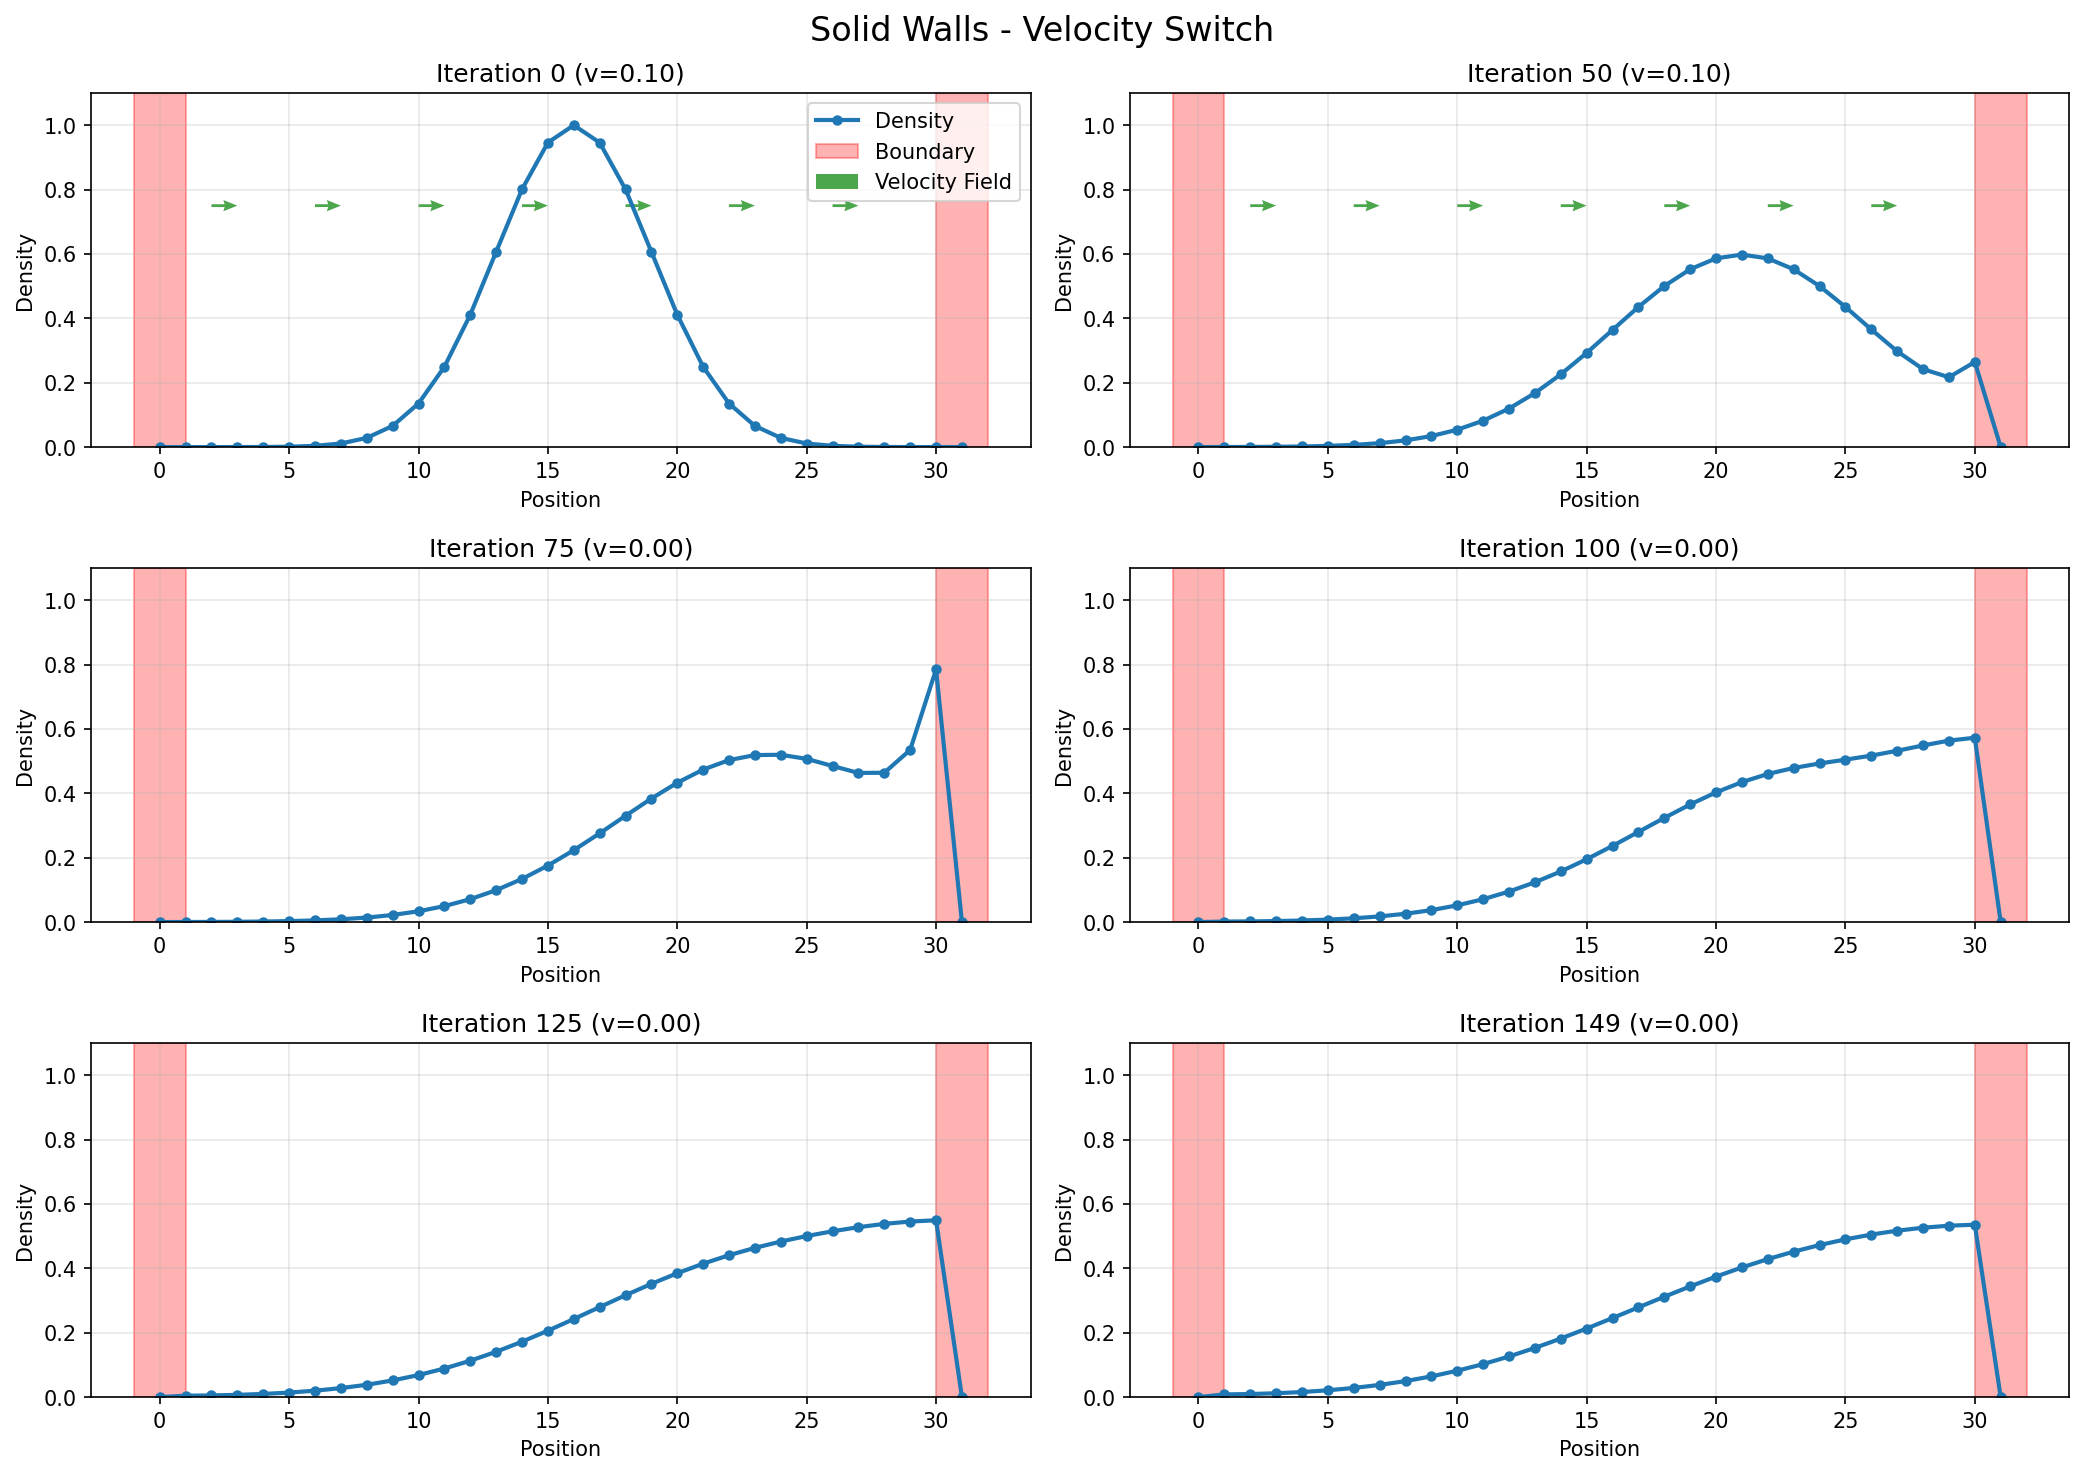
\includegraphics[width=14cm]{figures/snapshots.png}};

\end{tikzpicture}
\end{graphicalabstract}

%%Research highlights
\begin{highlights}
\item Generic framework for local, linear, norm-preserving boundary conditions in the Quantum Lattice Boltzmann Method
\item SVD-based decomposition combined with Linear Combination of Unitaries enables quantum implementation of non-unitary boundary operators
\item Pre-streaming integration of boundary and collision operators maintains 50\% success probability per iteration
\item Numerical validation demonstrates quantum-classical agreement up to numerical precision for 1D advection-diffusion with solid wall boundaries
\end{highlights}

\begin{keyword}
Quantum Lattice Boltzmann Method \sep Boundary Conditions \sep Linear Combination of Unitaries \sep Singular Value Decomposition \sep Advection-Diffusion Equation
\end{keyword}

\end{frontmatter}

%% \linenumbers

\section{Introduction}
Among methods for performing computational fluid dynamics (CFD) simulations on quantum computers, the Quantum Lattice Botlzmann Method (QLBM) is seen as a promising candidate and has been the subject of several recent works \citep{kocherla2024fully, xu2025improved, wang2025quantum, tiwari2025algorithmic}.

The classical Lattice Botlzmann Method (LBM) consists of two main steps: Collision, which is local but non-linear, and Streaming whch is linear but non-local.
Any worthwhile CFD simulation must also include boundary conditions in order to model relevant physical scenarios.
Authors usually implement specific boundary conditions directly into the circuits \citep{ljubomir2022quantum,jennings2026simulating,lee2025advanced}.

In this report, we propose a generic method for modelling \textbf{local, linear, norm-preserving} boundary conditions in a QLBM circuit.
The method is validated through a 1D advection-diffusion simulation with solid walls.
\section{Methodology}
\label{sec:method}

\subsection{Modeling Boundary Conditions}
In an LBM simulation, enforcing boundary conditions involves determining unknown incoming distributions at boundary nodes based on known outgoing distributions and other auxiliary information.
Depending on how the boundary is encoded into the lattice, LBM simulators distinguish between
\begin{itemize}
    \item \textbf{Wet-Nodes} The boundary conditions are applied directly on the fluid nodes at the boundary. This is usually done after streaming.
    \item \textbf{Link-Wise} The boundary conditions are applied between fluid nodes and solid nodes. This is usually done during streaming.
\end{itemize} \citep{olbug:18}.

Due to the linear constrains of quantum operations, we focused on modeling the unknown distributions as linear combinations of the known distributions at the boundary nodes.
This is a well known wet-node approach, detailed by \cite{zou1997pressure}.
Additionally, due to the norm-preserving nature of quantum operations, we restrict ourselves to boundary conditions that preserve the total density at the boundary node.
Mathematically, this can be expressed as:

\begin{equation}
f_i^{in} = \sum_j B_{ij} f_j^{out}
\end{equation}

Or in matrix form:
\begin{equation}
\mathbf{f}^{in} = B \cdot \mathbf{f}^{out}
\end{equation}

\subsection{Quantum Implementation via LCU and SVD}
Since the boundary matrix $B$ is generally non-unitary, it cannot be directly implemented as a quantum gate.
To address this, we can employ the Linear Combination of Unitaries (LCU) technique \citep{childs2012hamiltonian}
This is already used in many QLBM implementations to handle the collision step \citep{budinski2021quantum}.
Because the collision operator is diagonal, it was straightforward to express it as a linear combination of two unitaries:
\begin{equation}
C = \frac{1}{2} (C + i\sqrt{I - C^2}) + \frac{1}{2}(C - i\sqrt{I - C^2})
\end{equation} 

The Boundary operator $B$ is unfortunately not diagonal.
For simplicity, we opted to just decompose it using Singular Value Decomposition (SVD):
\begin{equation}
    B = U \Sigma V^{\dagger}
\end{equation}
where $U, V$ are unitary and $\Sigma$ is diagonal. Using this fact, we can decompose $\Sigma$ as a linear combination of two unitaries and distribute $U$ and $V^{\dagger}$ to obtain a linear combination for $B$:
\begin{equation}
    B = \frac{1}{2} (U (\Sigma + i\sqrt{I - \Sigma^2}) V^{\dagger} + U (\Sigma - i\sqrt{I - \Sigma^2}) V^{\dagger})
\end{equation}
This allows us to implement $B$ using one ancilla qubit with a 50\% success probability.

\subsection{Circuit Optimization}
As discussed, LCU is already employed for the collision step, already resulting in a 50\% success probability per iteration.
If we further add another LCU step for the boundary conditions, the overall success probability would drop to 25\%.

The idea here was to move the boundary conditions step before the streaming step, and combine the collision and boundary operators into a single matrix.
This is equivalent to considering the boundary conditions as a fundamental part of the collision process, instead of a separate step.
\begin{equation}
    C_{combined} =  B \cdot C
\end{equation}
We then perform SVD on this combined matrix $C_{combined}$. This maintains a single LCU step per iteration, preserving the 50\% success probability.

This shift does involve adjusting the boundary condition matrix to account for the fact that unknown distributions are now streamed immediately after being computed.
While we have not proven that it is always possible to rewrite a post-streaming boundary condition as a pre-streaming one, we have managed to do so for the case we tested.

\section{Experiments and Results}
\label{sec:exp}


\subsection{Experimental Setup}
The method was implemented using Qiskit \citep{qiskit2024} and validated using the statevector simulator.
The QLBM simulator was implemented by us previously, adapting and extending the work of \cite{wawrzyniak2025base}.
All code is open source and available at \url{https://github.com/widdrr/qlbm}

We validated the method using a 1D Advection-Diffusion setup.
This was chosen due to simplicity, but in theory nothing prevents the method from being applied to higher dimensions or more complex collision operators.
The simulation parameters were as follows:

\begin{itemize}
    \item \textbf{Lattice:} 1D grid, size 32.
    \item \textbf{Setup:} D1Q3 (Left, Rest, Right velocities).
    \item \textbf{Initial Condition:} Gaussian hill centered in the domain.
    \item \textbf{Velocity Field:} $u=0.1$ (rightward) for $t \in [0, 75]$, then $u=0$ for $t \in [75, 150]$.
    \item \textbf{Boundary Conditions:} Solid walls at both ends, populations that would stream into the boundary are instead redistributed to be stationary. Equations for right boundary:
    
    \[f_{-1}^{post} = f_{-1}^{pre} \]
    \[f_{0}^{post} = f_{0}^{pre} + 1.0 \cdot f_{1}^{pre}\]
    \[f_{1}^{post} = 0 \]
\end{itemize}

\subsection{Results}
We performed both a classical simulation (implementing the same matrix logic) and the quantum simulation (statevector simulator).
The classical simulation visually matched the expected behavior of a solid wall.

\begin{figure}[h]
    \centering
    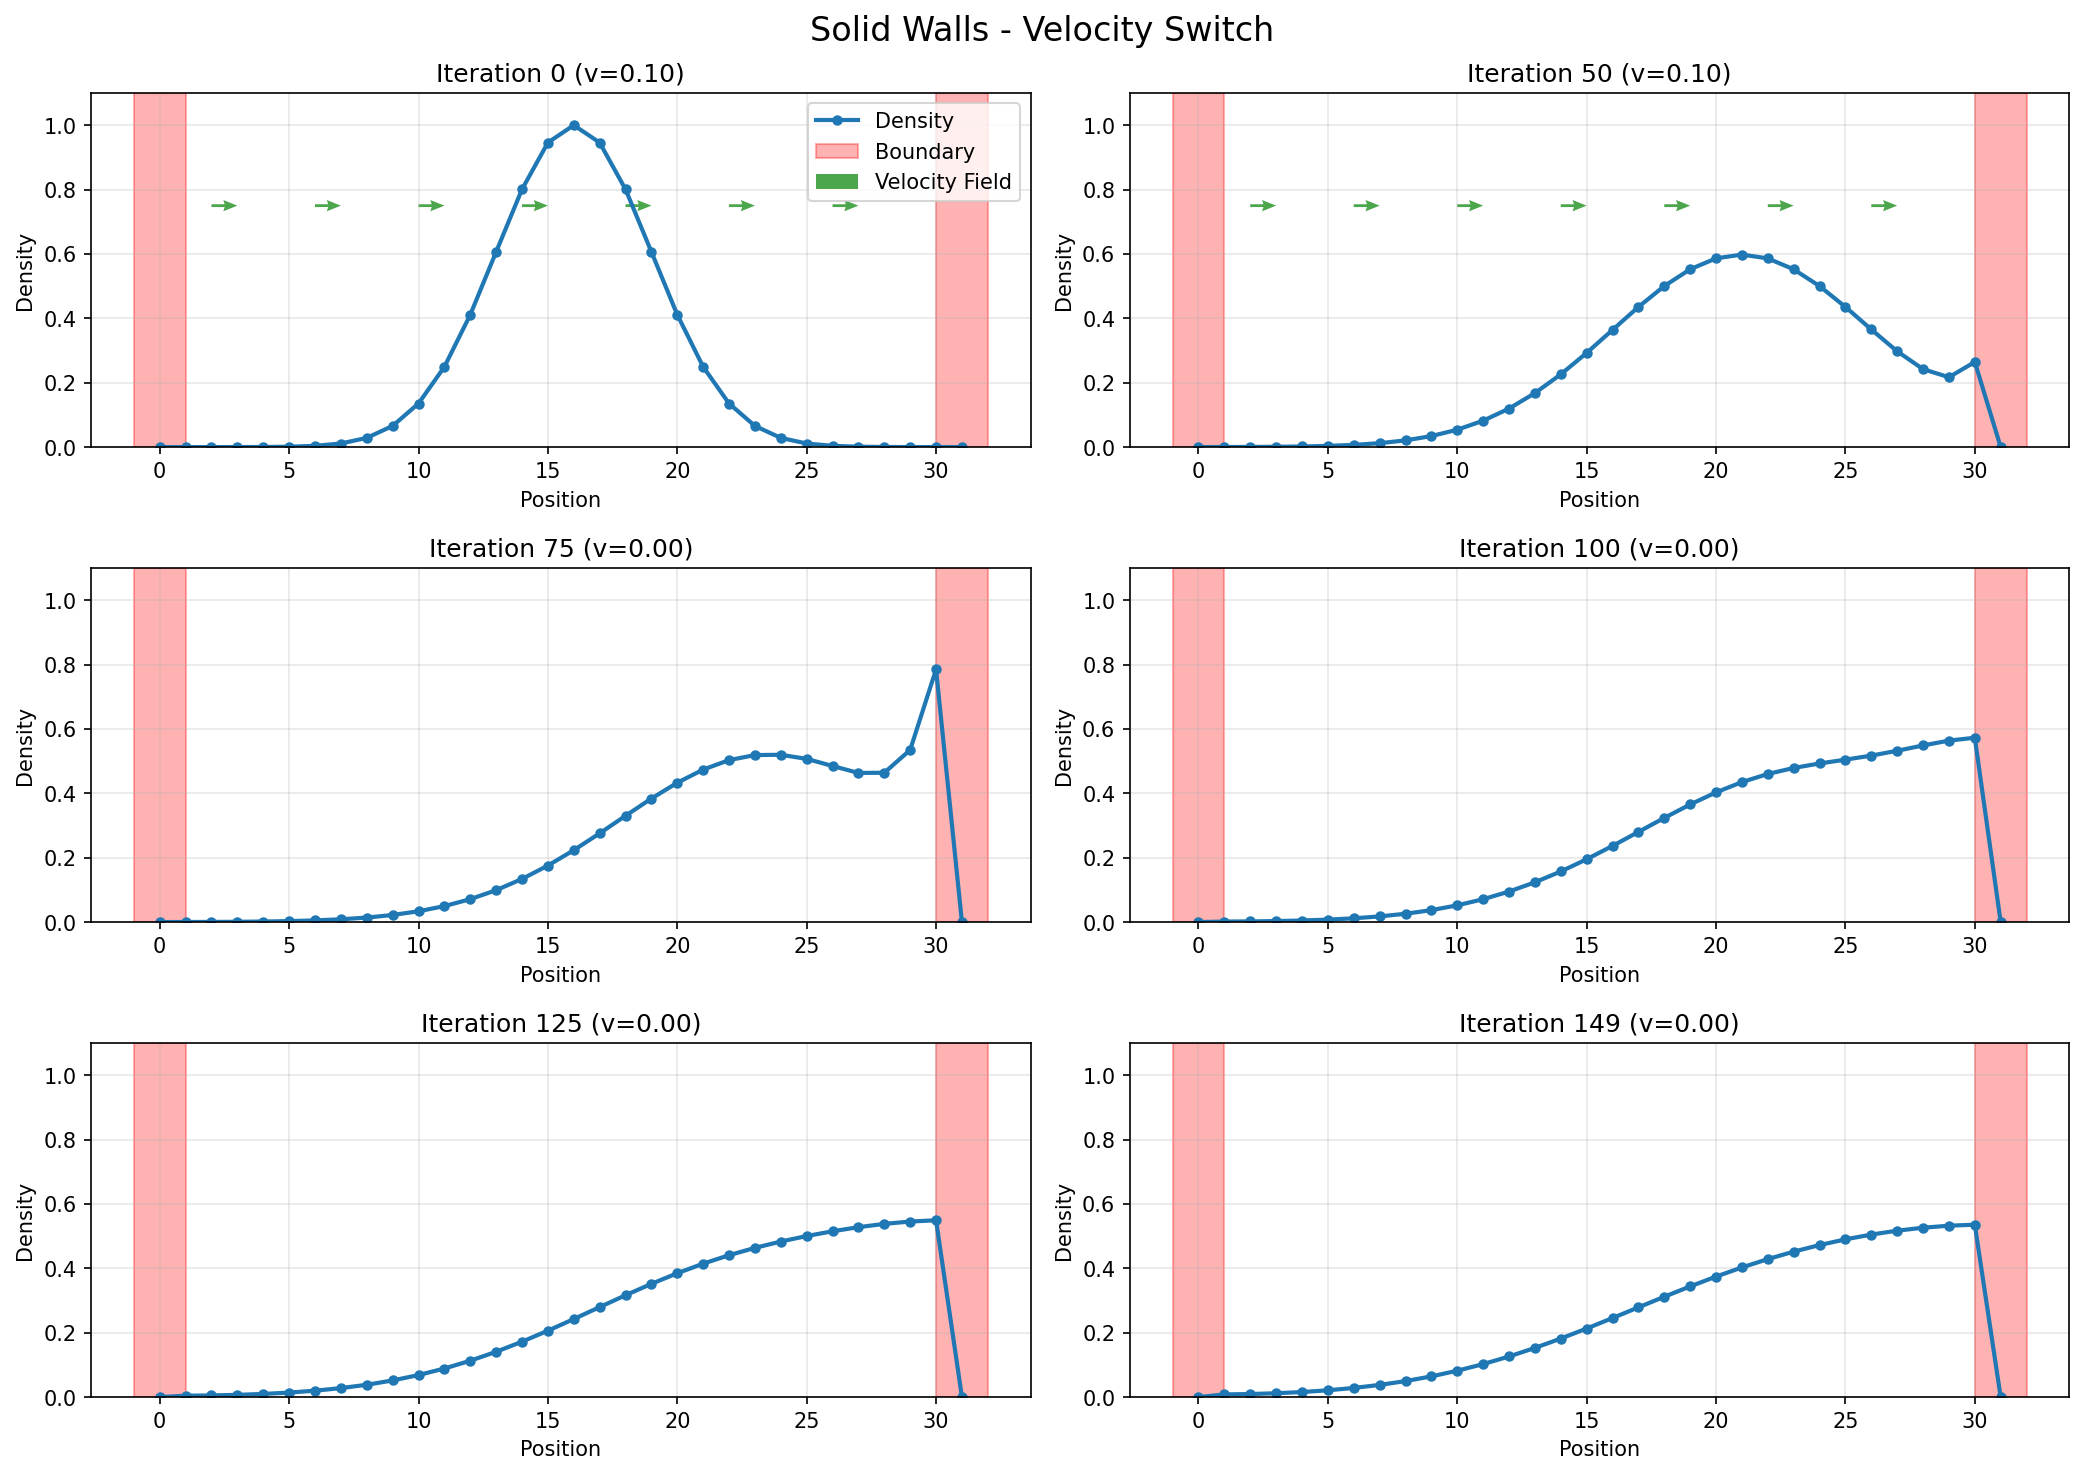
\includegraphics[width=0.8\textwidth]{figures/snapshots.png}
    \caption{Classical simulation results showing the Gaussian profile being contained by the solid walls. Given enough iterations, it would eventually flatten completely.}
\end{figure}

The quantum simulation was validated by computing the Root Mean Square Error (RMSE) between the classical and quantum results at each time step.

\begin{figure}[h]
    \centering
    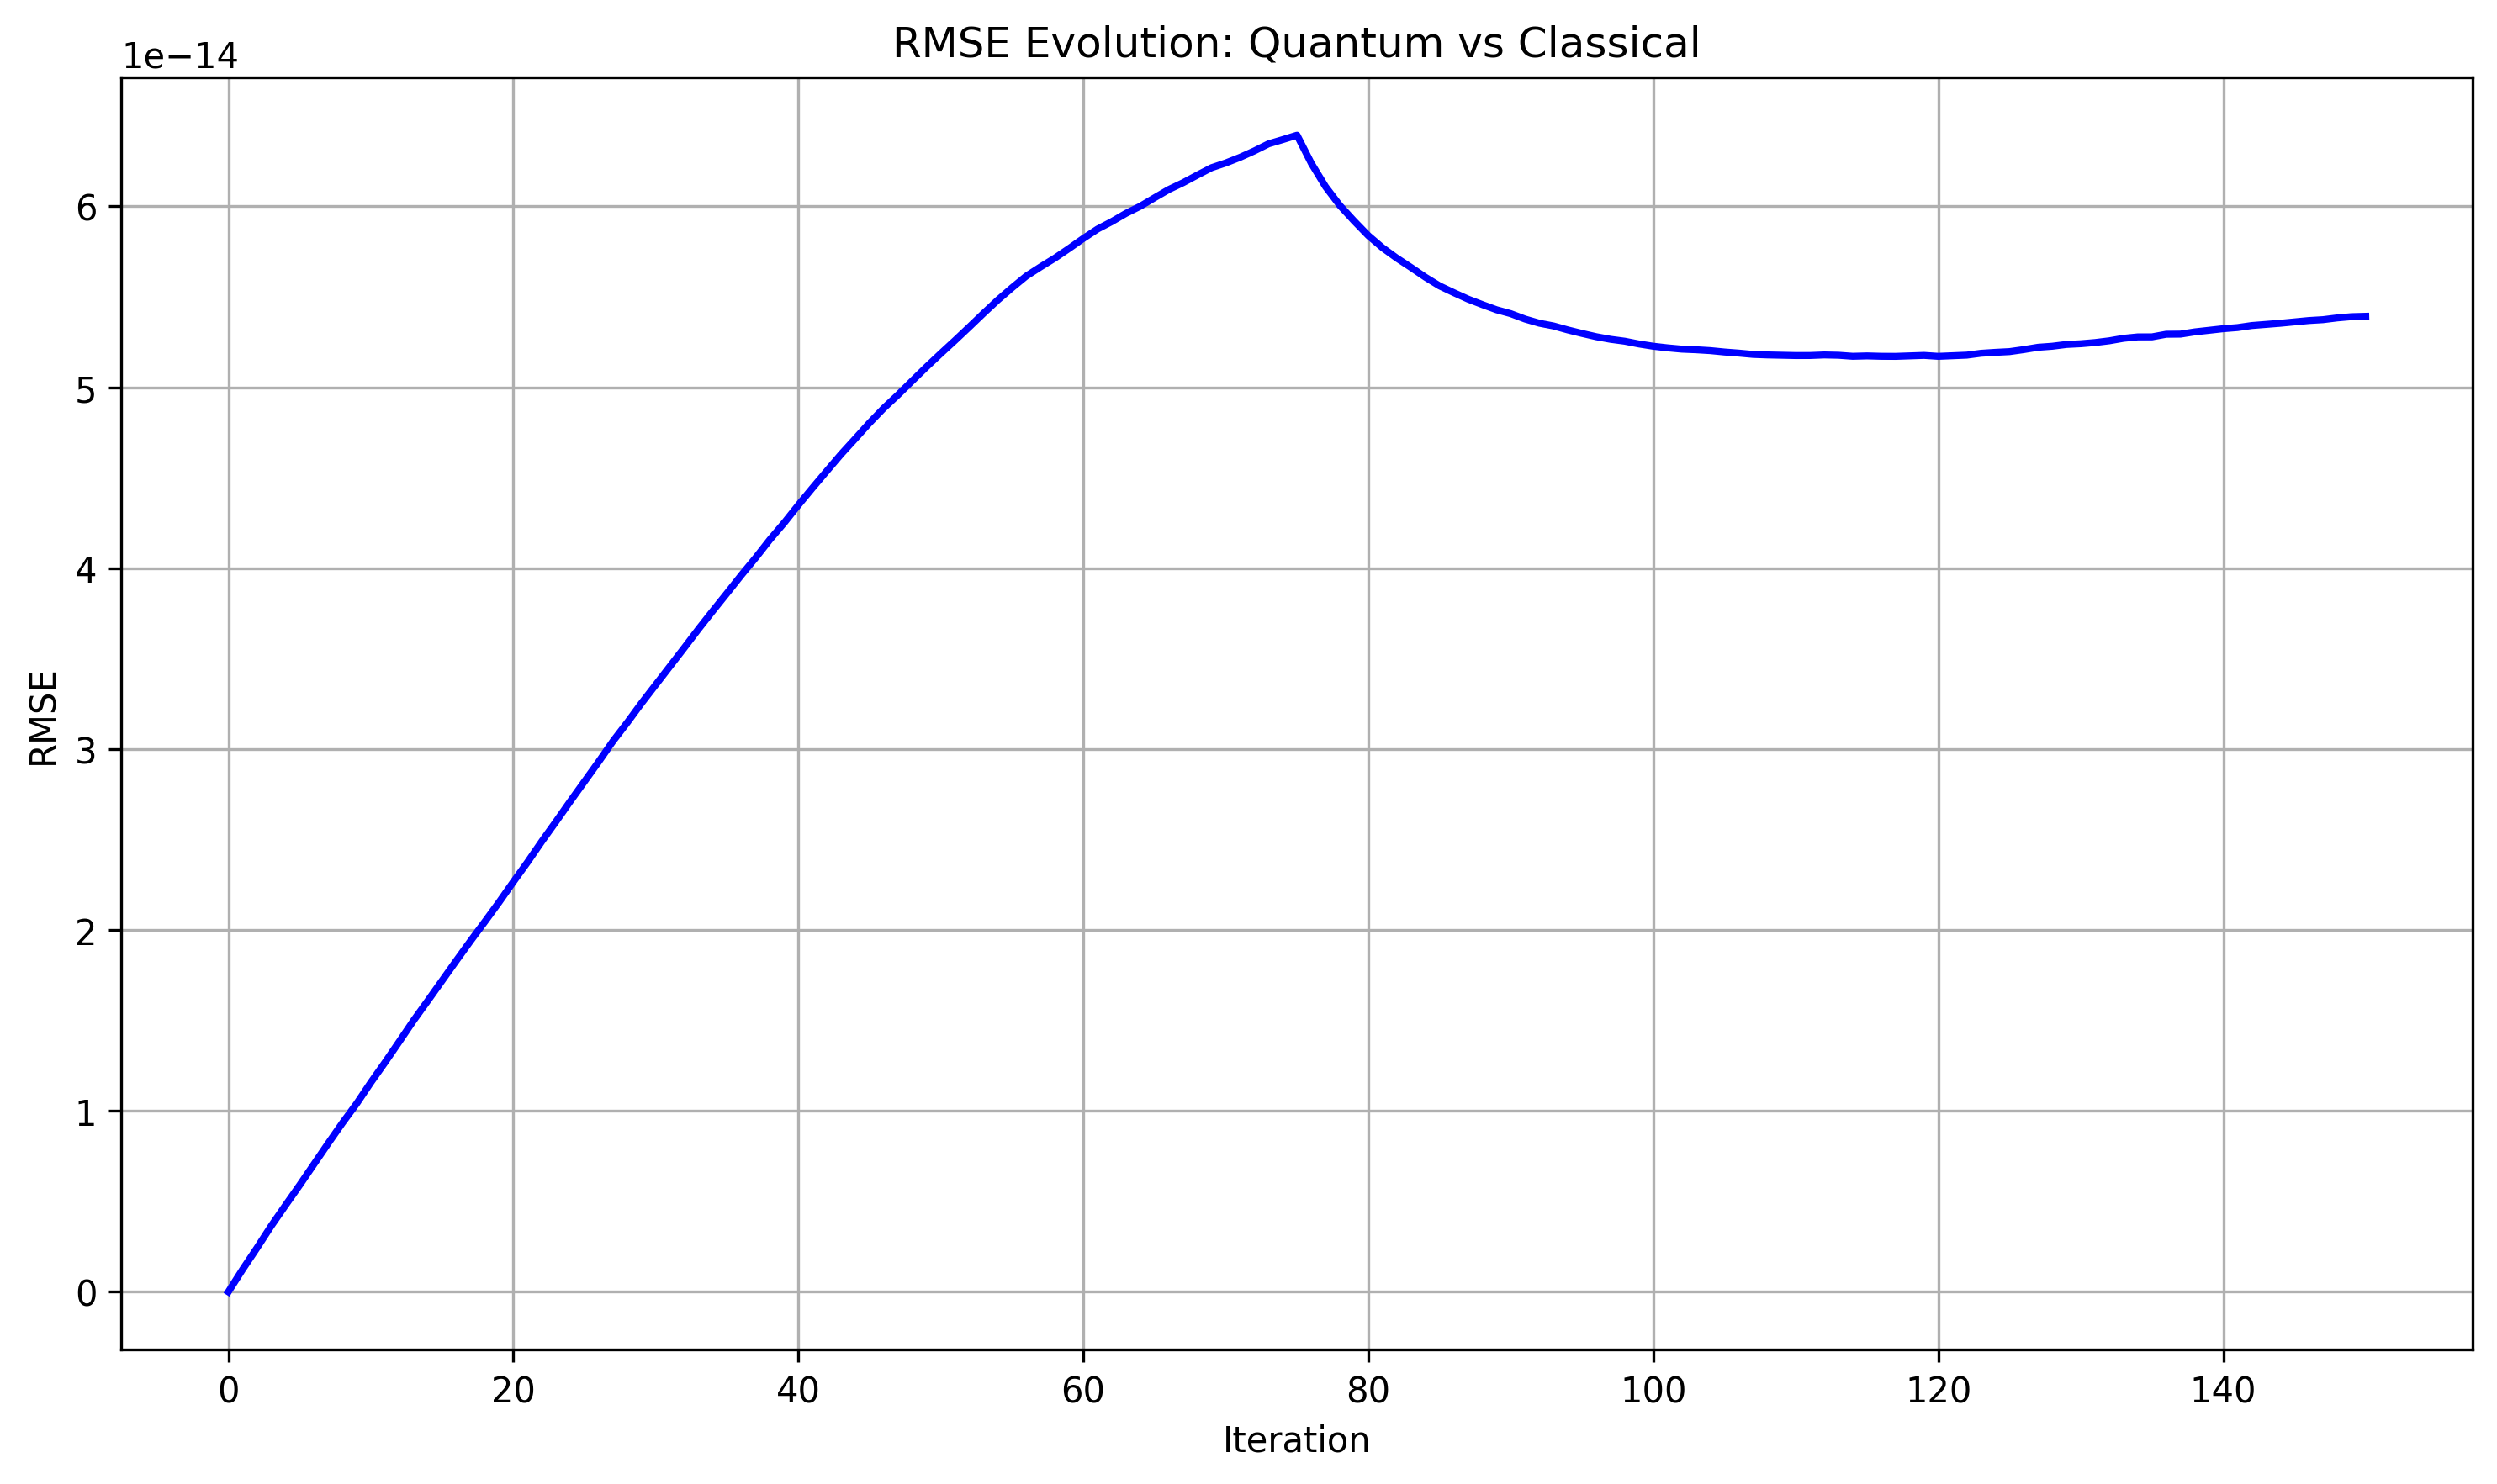
\includegraphics[width=0.8\textwidth]{figures/rmse_comparison.png}
    \caption{RMSE comparison between Classical and Quantum implementation demonstrating numerical precision agreement.}
    \label{fig:rmse}
\end{figure}

\section{Conclusion and Future Work}
\label{sec:concl}
We successfully demonstrated a generic method for implementing local, linear, norm-preserving boundary conditions in the QLBM.
The method leverages LCU and SVD to handle non-unitary boundary operators, and optimizes circuit design by combining collision and boundary steps.
Validation through a 1D advection-diffusion simulation with solid walls confirmed that the quantum implementation matches classical results within numerical precision.

There are plenty of directions for future work:
\begin{itemize}
    \item Investigating the kinds of boundary conditions that can be expressed using this method, and whether or not all post-streaming conditions can be rewritten as pre-streaming ones.
    \item Extending the method to support constants in the boundary equations, allowing for source and sink terms.
    \item Extending the method to support non-local boundary conditions that depend on multiple nodes.
    \item Testing the method in higher-dimensional simulations.
    \item Exploring other methods for the LCU decomposition that would avoid SVD.
\end{itemize}

\bibliographystyle{elsarticle-harv} 
\bibliography{references}

\end{document}
